
\section{Durchführung}
\begin{figure}[H]
  \centering
  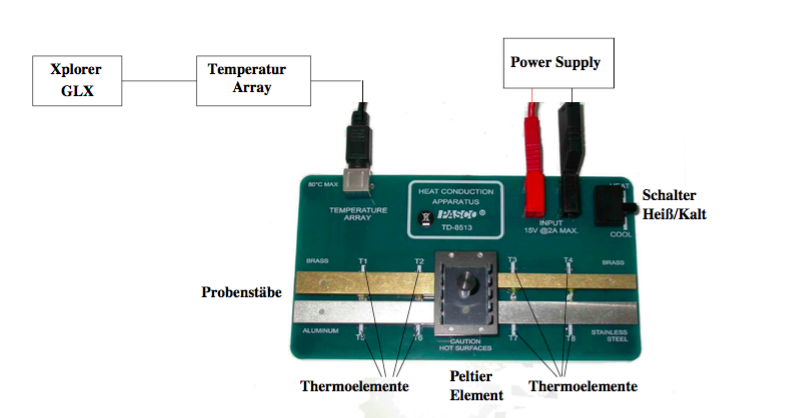
\includegraphics[height=7cm]{Aufbau.png}
  \caption{Versuchsaufbau \cite{skript}.}
  \label{fig:aufbau}
\end{figure}
In der Abbildung \ref{fig:aufbau} ist der Versuchsaufbau zu sehen. Hierbei sind die
4 zu untersuchenden Stäbe aus Messing(2x), Aluminium und Edelstahl auf der Platine befestigt,
wobei sich an jedem Stab je zwei Thermoelemete zur Temperaturmessung befinden. Diese
können automatisch vom GLX ausgelesen und die Messwerte per USB-Anschluss exportiert
werden.
In der Mitte befindet sich zudem ein Peltierelement, womit die Stäbe geheizt bzw. gekühlt
werden können, wobei darauf geachtet werden muss, dass der Schalter vor Versuchsbeginn auf
"COOL" steht.

\subsection{Statische Methode}
Im ersten Versuchsteil wird zunächst überprüft, ob alle 8 Thermoelemte auf dem GLX
angezeigt werden und die Abtastrate wird auf $\SI{5}{\second}$ gesetzt. Am Netzgerät wird eine Spannung
von $\SI{5}{\volt}$ bei maximalem Strom eingestellt und die Isolierung auf die Stäbe gelegt, um
den Temperaturaustausch mit der Umgebung zu minimieren. Anschließend wird der Schalter
auf “HEAT” gestellt und die Temperatur der Thermoelemte wird 30 min, bzw solange bis
eines der Thermoelemte über $\SI{45}{\celsius}$ anzeigt, gemessen. Nach der Messreihe
wird der Schalter wieder auf “COOL” gestellt und die Isolierung abgenommen.

\subsection{Dynamische Methode}
Im zweiten Versuchsteil wird die Spannung auf $\SI{8}{\volt}$ erhöht und die Abtastrate
auf $\SI{2}{\second}$ herabgesetzt. Die Messung kann beginnen, sobald alle Thermoelemte
maximal $\SI{30}{\celsius}$ anzeigen. Dann wird die Isolierung wieder auf die Stäbe gelegt
und das Peltier-Element periodisch zunächst für $\SI{40}{\second}$ auf “HEAT” und dann
für $\SI{40}{\second}$ auf “COOL”. Dabei werden mindestens 10 Perioden gemessen und anschließend
wird die Isolierung wieder entfernt und das Gerät in der Stellung “COOL” belassen.
\\
\noindent Sind die Stäbe wieder hinreichend abgekühlt (unter $\SI{30}{\celsius}$), wird eine analoge
Messung mit einer Periode von $\SI{200}{\second}$, also einem Umschalten alle $\SI{100}{\second}$
durchgeführt. Es wird solange gemessen, bis mindestens 10 Perioden aufgenommen sind oder eines
der Thermoelemte $\SI{30}{\celsius}$ überschreitet.
